\documentclass[a4paper,11pt]{article}
\usepackage[margin=2cm]{geometry}
%% Language and font encodings
\usepackage[english]{babel}
\usepackage[utf8x]{inputenc}
\usepackage[T1]{fontenc}
% \usepackage{microtype}      % fine pdf font control

\usepackage[scaled=0.92]{helvet} \renewcommand{\familydefault}{\sfdefault}
\usepackage{xcolor} % -- loaded by tikz


% \usepackage[colorlinks=true]{hyperref}
\usepackage[colorlinks = true,
            linkcolor = blue!50!black!50,
            urlcolor  = blue!50!black!50,
            citecolor = blue!50!black!50,
            anchorcolor = blue!50!black!50]{hyperref}
\usepackage{natbib}
\usepackage{apalike}
\usepackage{graphicx}
\usepackage{verbatim}

\usepackage{float}
\usepackage{wrapfig}

\usepackage[font={footnotesize}]{caption}

\makeatletter
\renewcommand\paragraph{\@startsection{paragraph}{4}{\z@}%
            {-2.5ex\@plus -1ex \@minus -.25ex}%
            {1.25ex \@plus .25ex}%
            {\normalfont\normalsize\bfseries}}
\makeatother
\setcounter{secnumdepth}{4} % how many sectioning levels to assign numbers to
\setcounter{tocdepth}{4}    % how many sectioning levels to show in ToC
\usepackage[tiny]{titlesec} % format section titles
\def\headfmt{\color{blue!50!black!50}\bfseries}
\titleformat*{\section}{\headfmt}
\titlespacing*{\section}{0pt}{*1}{*0}[-4em]
\titleformat*{\subsection}{\headfmt}
\titlespacing*{\subsection}{0pt}{*0.5}{*0}
\titleformat*{\subsubsection}{\headfmt}
\titlespacing*{\subsubsection}{0pt}{*0}{*0}
\titleformat*{\paragraph}{\headfmt}
\titlespacing*{\paragraph}{0pt}{*0.5}{*0}

\title{Case for Support}
\author{}

\begin{document}

% \maketitle

\tableofcontents
    
\newpage

\setcounter{page}{1}

\section*{\large Case for support}
\vskip 0.5ex
We propose to extend, enhance, maintain and support \textbf{Bonsai}, a fully
integrated software environment to \textbf{enable cutting-edge reproducible
  laboratory systems neuroscience experiments in animal models}, with a
particular emphasis on \textbf{machine-intelligence-enabled, real-time
  neuroinformatics} methods.

\section{Background: real-time neuroinformatics and control in behavioural systems
  neuroscience}
  
\setlength{\columnsep}{1em}
\begin{wrapfigure}{R}{0.5\textwidth}
    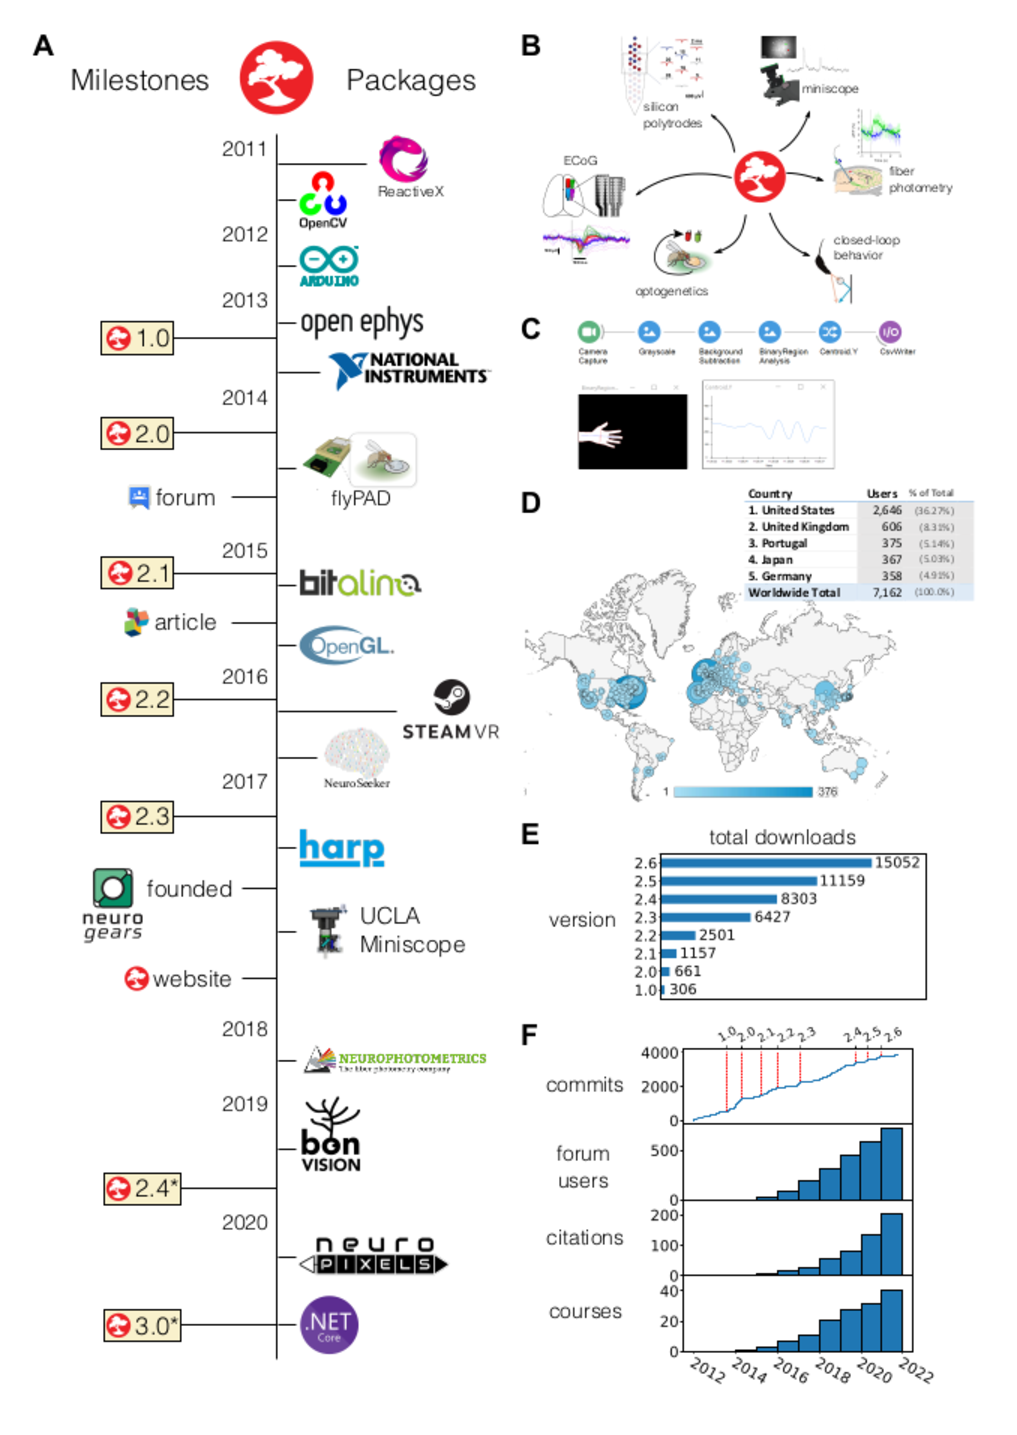
\includegraphics[width=0.5\textwidth]{figures/roadmap-bbsrc-2x_cropped.pdf}

  \caption{Bonsai development timeline and community adoption. (A) Timeline of
    milestones and landmark package releases. (B) Example capabilities 
    within Bonsai. (C) Bonsai workflow for tracking the position of objects
    in a video. (D) Worldwide
    distribution of visitors to the bonsai-rx.org website. (E)
    Number of downloads for each Bonsai version. (F) Cumulative number of
    registered forum users, citations of the main publication, and number of
    training events, by year (bottom panels), versus release and development
    cycle (top panel), measured in commits to main repository. 
    % Click on the image to see its online version.
    }

  \label{fig:bonsai}
\end{wrapfigure}

To understand the neural basis of behaviour, experiments need to control and quantify animal behaviour whilst recording, and often manipulating, neural activity. 
%
Powerful experimental designs require behavioural feedback (e.g.\ reward, lights, sounds, actuated
devices) or neural perturbation (e.g.\ using light-sensitive polarising
molecules) that depend on real-time behaviour or neural state.
%
It has also become increasingly apparent that the neural signals that
drive complex behaviour are manifest in a broad population of neurons rather
than in single cells. Current neural recording emphasises high-dimensional
signals from 100s to 1000s of neurons monitored using multi-electrode arrays or cellular-resolution imaging, with a wide array of probe configurations and neural targets.
%
\textbf{This complexity of experiments limits the potential for database-driven progress in systems neuroscience}. The number of possible experiments is astronomical, and new questions are typically answered by designing and conducting new experiments rather than mining data from old ones.

At present, progress in the field is held back by the challenge of designing and implementing new experimental protocols, and the difficulty of integrating state-of-the-art data processing and neuroinformatics into custom experimental designs.
%
\textbf{Reproducibility}, in particular, depends on the availability of
standardised tools for experimental control and analysis, shared between
laboratories \citep{baker16,ioannidis05}. Although such tools exist in genetics, astronomy, physics and medicine (Fish et al., 2016; Abdalla et al., 2018, CERN Education, Communications and Outreach Group, 2018, Dickinson et al., 2016, Bycroft et al., 2018), they are mostly lacking in neuroscience, with documented consequences for the reliability of ``discoveries'' (Baker, 2016; Botvinik-Nezer et al., 2020; Button et al., 2013). 


\textbf{Bonsai}~\citep{lopesEtAl15,lopesAndMonteiro21} is a free and open-source visual programming language developed 
in response to these challenges.
% ~\citep{lopesEtAl15,lopesAndMonteiro21} is a free and open-source visual
% programming language that 
Its design emphasises performance, flexibility, and ease-of-use,
allowing scientists with no previous programming experience to quickly develop
their own high-performance data acquisition and experimental control systems.
Bonsai combines a high-level event algebra for data streams with an integrated
development environment (IDE) and an extensive library of plugins supporting
multiple hardware and software packages used by the neuroscience research
community (Figure~\ref{fig:bonsai}A-B).
%
A Bonsai graphical program consists of one or more source data streams (e.g.\ neural activity, video, audio, sensors, etc)
and several interconnected operators that transform input to output
datastreams (Figure~\ref{fig:bonsai}C).

% I think we've said something similar in the first para  - m.
%
% Standard software tools for data analysis (ImageJ, MATLAB, R, etc.) have
% transformed progress inf increasingly “data-rich” sciences. However,
% equivalent standardised software tools for data acquisition and control of
% animal behaviour in neuroscience experiments are still lacking. Life science experiments demand
% a combination of multiple instrumentation and control technologies, for both
% behavioural and physiological investigations. The growing complexity on both the
% amount of data that is collected, and the rich conditions under which behaviour
% must be explored, place an increasing burden on experimenters to integrate
% highly specialised equipment in unique configurations, while often lacking
% expertise in the relevant engineering fields.



Bonsai has been adopted in hundreds of laboratories worldwide and has the largest user base in the systems neuroscience community (Figure~\ref{fig:bonsai}D-F).  In the last year alone, more than 1,000 new users incorporated Bonsai into their experimental protocols. The rapid rate of adoption of Bonsai in non-programmer experimental
labs highlights the need for accessible design tools that enable
state-of-the-art technology but also allow researchers to stay in control and flexibly
change their experimental paradigms.  Many open-source software tools are
either inaccessible to non-programmers, or too constrained to be of general use
outside their narrow domain of application. Bonsai has been successful because
it bridges this gap.

Bonsai also supports the growing wave of foundational
open hardware initiatives, such as OpenEphys \citep{siegleEtAl17} and UCLA
Miniscope~\citep{caiEtAl16}, allowing these tools to be quickly combined and integrated into new experiments~\citep{buccinoEtAl18}.
%
Bonsai has been adopted in large neuroscience undertakings like the
International Brain
Laboratory \footnote{internationalbrainlab.com/}
and the Allen Institute for Brain
Science\footnote{https://alleninstitute.org/what-we-do/brain-science/}.
%
Key to the wide adoption is the reproducibility that Bonsai ensures.  Data acquisition and experimental control protocols can be 
replicated in any laboratory just by sharing a Bonsai configuration file. 
%
% LEAVE OUT FOR THIS GRANT:
% More recently, Bonsai has started to expand outside the domain of neuroscience
% into biomedical research and biotechnology tool development, and even outside
% academia into public outreach and education programs.




Bonsai achieves robust behavioural control, hardware interaction and signal acquisition while ensuring remarkable ease of use.  The proposed project will provide valuable enhancements to the existing codebase.  We will develop, test and deploy a new software workflow making it possible to incorporate external packages into Bonsai's C\#-based environment.  Building on this new extensibility, we will then incorporate a suite of machine-learning-driven analysis tools into the Bonsai environment.  These added capabilities will allow  video-based behavioural analysis as well as real-time interfacing of population-scale activity with laboratory control.  In parallel we will develop the infrastructure needed to evaluate competing data analytic approaches within a single experimental framework

The proposed project will \textbf{enhance, reinforce and support} this key neuroinformatics
resource to streamline \textbf{reproducible experimental design, data collection and analysis}, while making \textbf{standardised implementations of cutting-edge machine-learning methodologies} widely available to the community, potentially creating the most powerful experimental
control and analysis tool available to neuroscientists, psychologists and
ethologists worldwide.

\subsection*{Other resources in the subject area}

The space of technologies serving experimental control and behaviour monitoring
is large, and is traditionally occupied either by domain-specific graphical
user interfaces for control and recording of specific devices and experiment
types (e.g.\ Open Ephys
GUI\footnote{https://open-ephys.org/gui/},
Miniscope DAQ
Software\footnote{https://github.com/Aharoni-Lab/Miniscope-DAQ-QT-Software})
or by real-time control frameworks for specifying task logic using state
machine or similar formalisms (e.g. NIMH ML\footnote{https://monkeylogic.nimh.nih.gov/},
pyControl\footnote{https://pycontrol.readthedocs.io/en/latest/},
Autopilot\footnote{https://docs.auto-pi-lot.com/en/latest/},
Sanworks\footnote{https://sanworks.io/index.php}).
These dedicated interfaces are typically very comfortable for experimenters
operating within the specific domain that the tool is designed for, but tend to
become unwieldy when there is a need to introduce a new device or variation of
a task which is outside the scope of the framework. The alternative is to use a
more general programming language like Python or MATLAB, with the disadvantage
of the code being harder to understand, maintain, and change. Programming
languages like LabVIEW straddle the middle ground and provide a high-level and
flexible visual interface for composing data acquisition and control systems
themselves. Unlike Bonsai, however, the graphical elements of LabVIEW are
heterogeneous and very fine grained, creating the need for long and complicated
logical structures to implement even a simple experimental control system. By
providing an extremely simple, yet flexible, visual syntax, Bonsai opens the
opportunity even for complete non-programmers to design and successfully
customize relatively complex experiments from the ground up. It is mostly this
capability which has made Bonsai so attractive as a standard tool in
experimental neuroscience.




% A central goal of the software resource proposed here is to address this
% problem, by extending Bonsai~(an experimental control software ecosystem;
% Figure~\ref{fig:bonsai} and Section~\ref{sec:bonsai}) with state-of-the-art
% online (and offline) data analysis methods
% (Figure~\ref{fig:proposedBonsaiExtensions} and
% Section~\ref{sec:functionality}).
% Bonsai is unique amongst experimental control systems in that
% it allows users with no programming expertise to design and implement
% sophisticated experiments.
%
% The latest Its large and rapidly growing community of users demonstrates the demand for such software resources.
%

% With the proposed enhancements, users of Bonsai will be able to use sophisticated \textbf{machine-learning methods} to
% control their experiments and analyse their data. This \textbf{democratisation}
% of machine learning functionality will allow scientists without computational
% skills to control sophisticated experiments and analyse their data in
% unprecedented ways, which will facilitate \textbf{advances in explaining how the
%   brain gives rise to behaviour}.



% \subsection{Bonsai}
% \label{sec:bonsai}




% 1. Develop, test and deploy a new software workflow to incorporate external packages into Bonsai's C# environment.

% 2. Incorporate a suite of machine-learning-driven analysis tools into the Bonsai environment to implement:
% 2a. video-based  behavioural analysis
% 2b. real-time interfacing of population-scale activity with laboratory control  
% 2c. evaluate competing data analytic approaches within a single experimental framework

\section{Details of proposed resource enhancements}

We will enhance Bonsai's extensibility in two ways.
%
First, we will create a new package infrastructure to enable the integration of software objects implemented in non-native languages into Bonsai.
%
Second, we will create a new general abstraction framework within Bonsai suited to the implementation and application of data analytic algorithms.
%
Both frameworks will expose public interfaces available to all developers within the user community, thus simplifying and accelerating community-driven development.

Furthermore, we will build on these extensibility developments to implement a suite of advanced machine intelligence neural data analysis methods that will be made available as one or more core Bonsai packages.

\subsection{Extensions to incorporate non-native code packages into Bonsai}

Bonsai is designed to be extensible and is distributed with a package-management framework that controls installation of optional core packages as well as user-contributed extensions.
%
However, extensions must be written in Bonsai's native C\# programming language.
%
This restricts the range of potential contributors to the ecosystem.
%
It also hinders incorporation of published analytic tools, many of which are implemented within other interpreted language systems such as Python, R, or MATLAB.  
\begin{wrapfigure}{R}{0pt}
  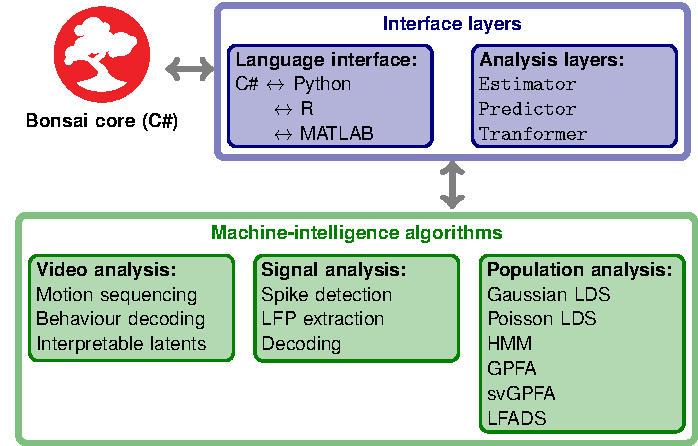
\includegraphics[width=0.5\textwidth]{figures/extensions.pdf}%
%   % \documentclass{standalone}
% %% Fonts, etc.

% %% Language and font encodings
% \usepackage[english]{babel}
% \usepackage[utf8x]{inputenc}
% \usepackage[T1]{fontenc}

%  \usepackage[scaled=0.92]{helvet} \renewcommand{\familydefault}{\sfdefault}
%  \usepackage{xcolor}
% % \usepackage{soul} % \ul \st \hl


% %% Maths

% % \usepackage{amssymb,amsmath}
% % \input m.macros
% % \input m.symbols


% %% Graphics

% \usepackage{graphicx,tikz}
% \usetikzlibrary{positioning}
% \usetikzlibrary{fit}
% \usetikzlibrary{calc}






% %% Document
% \begin{document}

\begin{tikzpicture}[
    ML/.style={text width=10em, rounded corners,
      fill=green!50!black!30, draw=green!50!black, very thick},
    Ext/.style={text width=10em, rounded corners,
      fill=blue!50!black!30, draw=blue!50!black, very thick}
    ]

  \node[text width=10em, font={\bf}, align=center]
       (bonsai)
       {\includegraphics[width=7em]{bonsai-lettering}\\
         Bonsai core (C\#)};

       
 \coordinate [below = 5em of bonsai.south] (A);

  \node[below left=0 and 1em of A, Ext]
       (lang)
       {\textbf{Language interface:}\\
         C\# $\leftrightarrow$ Python\\
         $\qquad \leftrightarrow$ R\\
         $\qquad \leftrightarrow$ MATLAB
       };


  \node[below right=0 and 1em of A, Ext]
       (abstr)
       {\textbf{Analysis layers:}\\
         \texttt{Estimator}\\
         \texttt{Predictor}\\
         \texttt{Tranformer}};

  \node[above=1ex of A, text=blue!50!black, font={\bf}, inner sep=0]  (intr) {Interface layers};

  \node[fit=(lang) (abstr) (intr), line width=1mm, draw=blue!50!black!50, rounded
    corners, inner sep=1ex] (intr box) {};

 \coordinate [below = 12em of A] (B);


 \node[below=0 of B, ML]
       (signal)
       {\textbf{Signal analysis:}\\
         Spike detection\\
         LFP extraction\\
         Decoding};

  \node[below left=0 and 1em of signal.north west, ML]
       (video)
       {\textbf{Video analysis:}\\
         Motion sequencing\\
         Behaviour decoding\\
         Interpretable latents};
       
       
  \node[below right=0 and 1em of signal.north east, ML]
       (dimred)
       {\textbf{Population analysis:}\\
         Gaussian LDS\\
         Poisson LDS\\
         HMM\\
         GPFA\\
         svGPFA\\
         LFADS};

  \node[above=1ex of B, text=green!50!black, font={\bf}, inner sep=0] (ml)
       {Machine-intelligence algorithms};

  \node[fit=(video) (signal) (dimred) (ml), line width=1mm, draw=green!50!black!50, rounded
    corners, inner sep=1ex] (ml box) {};


  \draw[<->, line width=1mm, gray] (bonsai) -- (intr box);

  \draw[<->, line width=1mm, gray] (intr box) -- (ml box);

  
  

  %% \node[below = 15em of bonsai, ML]
  %% (compare)
  %%      {\textbf{Method comparison}};
       
\end{tikzpicture}

% \end{document}

% Local Variables:
% mode: latex
% eval: (set-fill-column 80)
% End:

  \caption{Proposed extensions to Bonsai}
  \label{fig:proposedBonsaiExtensions}
\end{wrapfigure}

We will extend the Bonsai package interface to allow direct interaction with the runtime execution environments that implement these common languages.  
%
Where possible, the extensions will be based on existing pipeline tools that allow C\#-based programs to interact with a number of alternative run-time engines.
%
These include:
%
Python.NET\footnote{https://github.com/pythonnet/pythonnet},
%
R.Net\break \footnote{https://github.com/rdotnet/rdotnet}
%
and the native .NET interface shipped with MATLAB.
% \footnote{https://uk.mathworks.com/help/matlab/matlab\_external/using-net-from-matlab-an-overview.html}.  TOO LONG
%
If necessary, we will also incorporate direct inter-runtime communication using the messaging library ZeroMQ\footnote{https://zeromq.org/}.

\subsection{General abstraction framework for data processing}
\label{sec:generality}

To avoid the need to re-implement a single data analysis algorithm to handle multiple different data types we will create a set of abstract machine-intelligence operators in Bonsai that can be configured to map between data substrates and ML algorithms.
%
The planned abstraction layer is based on the successful \texttt{scikit-learn} Python
library \citep{buitinckEtAl13}.
%
By analogy to the interfaces provided by this library we will introduce three types of Bonsai operator: \texttt{Estimator} objects for building and fitting models, \texttt{Predictor} objects for making predictions and \texttt{Transformer} objects for converting data.
%
Interactions between these different object types will allow a single algorithm class (implemented by \texttt{Estimator} and \texttt{Predictor} operators) to act on many different data streams.
%
% An example closed-loop architecture allowing online control of a compu|ter cursor with neural activity is shown in Figure~\ref{fig:proposedBonsaiExtensions}b. The Bonsai
% graphical program for this system is given in Figure~\ref{fig:proposedBonsaiExtensions}c. The
% objects instantiating the SpikeThresholdDetector, the KiloSortSpikeSorter and
% GPFAlatentsExtractor implement the \texttt{Transformer} interface (blue),
% and the object instantiating the TimeSeriesForestClassifier implements the
% \texttt{Predictor} interface (green; Figure~\ref{fig:proposedBonsaiExtensions}c, top).
% %
% While the parameters for the SpikeThresholdDetector and the KiloSortSpikeSorter may
% be set manually by the user, the parameters of
% the GPFAlatentsExtractor can be learnt offline in an unsupervised way using an
% \texttt{Estimator} (red) in a second pipeline
% (Figure~\ref{fig:proposedBonsaiExtensions}c, middle).
% Finally, the parameters of the TimeSeriesForestClassifier can also be learnt
% offline, but in a supervised way, using another \texttt{Estimator} in a third
% pipeline (Figure~\ref{fig:proposedBonsaiExtensions}c, bottom).






% This initial set of methods should demonstrate to Bonsai users, and to
% machine-learning methods developers, the potential of embedding
% machine-learning functionality into the experimental control loop. We propose
% user engagement activities to expose both of these groups to this
% potential (Section~\ref{sec:userEngagement}).  As data-analysis method
% developers recognise this opportunity, they will become interested in
% contributing their methods to the Bonsai ecosystem, ensuring the
% \textbf{long-term sustainability} of the proposed resource.

% Adding machine learning functionality to the experimental control loop will
% make possible the implementation of experiments with unprecedented levels of
% control. Moreover, equipping experimental scientists without programming
% experience with machine learning tools will considerably increase the
% application of machine learning to the biosciences, which most probably will
% translate into groundbreaking scientific discoveries.



% Developers of advanced data-analysis methods should become interested in
% integrating them into the Bonsai ecosystem, as it will allow their methods to
% reach the wide Bonsai user community. In addition this integration will enable
% method developers to easily compare the performance of their methods with
% that of many methods previously integrated into the Bonsai ecosystem. Method
% developers will thus become a new type of Bonsai users, which will contribute
% to the \textbf{sustainability} of the proposed resource beyond the period of
% BBSRC-BBR funding.

% Scientific advances rely on \textbf{reproducibility}, which in turn depends on standardized tools for experimental control and analysis, shared between laboratories (Baker, 2016; Ioannidis, 2005). Although such tools exist in genetics, astronomy, physics and medicine (Fish et al., 2016; Abdalla et al., 2018, CERN Education, Communications and Outreach Group, 2018, Dickinson et al., 2016, Bycroft et al., 2018), they are mostly lacking in neuroscience, which in itself suffers from a paucity of reproducible discoveries (Baker, 2016; Botvinik-Nezer et al., 2020; Button et al., 2013). Bonsai is an excellent tool for reproducible data acquisition and experimental control. For example, an experiment implemented in Bonsai can be replicated in
% any laboratory by just sharing a Bonsai configuration file. With the addition of the proposed machine learning functionality Bonsai will extend this
% reproducibility to the domain of data analysis
% (Section~\ref{sec:reproducibility}).


% \begin{figure} \begin{center}

%     \href{http://www.gatsby.ucl.ac.uk/~rapela/bbsrc-bbr21/proposed_bonsai_extensions_combined.png}{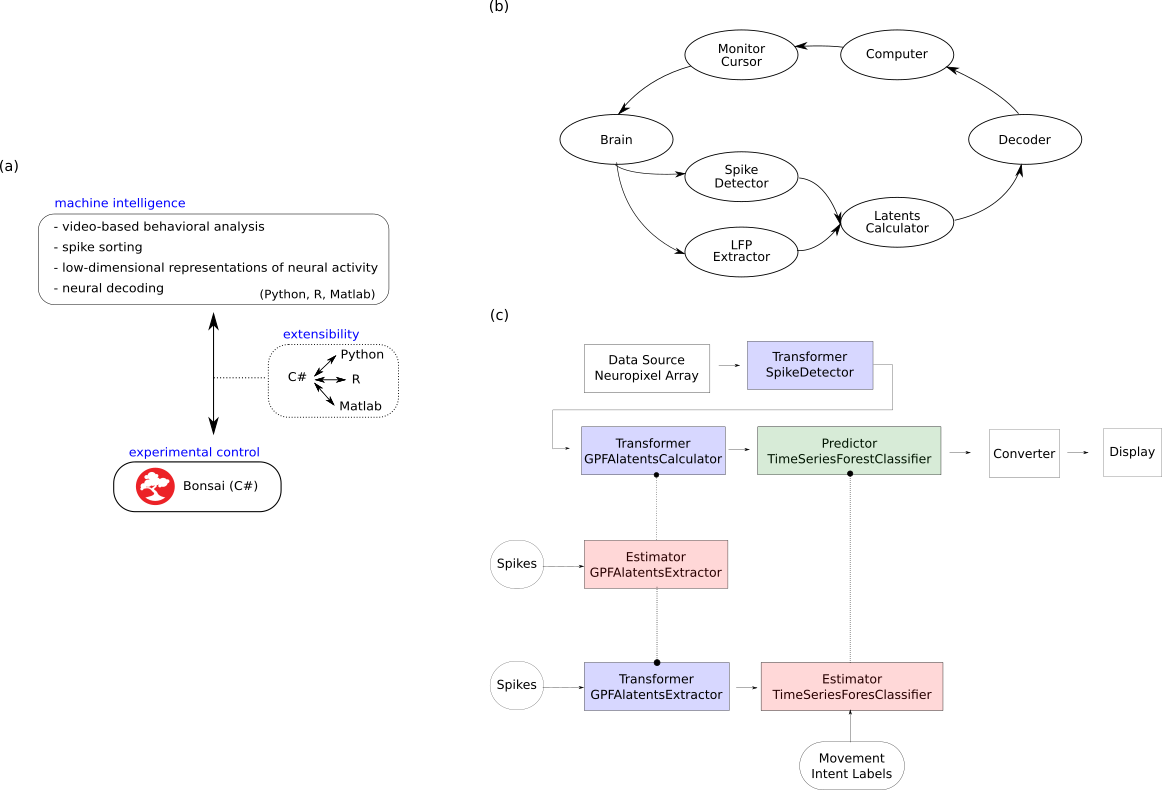
\includegraphics[width=5in]{figures/proposed_bonsai_extensions_combined.png}}

%     \caption{Extensions to Bonsai. (A) we propose to integrate machine learning
%     functionality into the experimental control loop by building software
%     infrastructure to allow Bonsai to communicate with existing machine
%     learning software written in Python, R and Matlab. (B) flow chart
%     representing the BCI application that we propose to implement with the
%     machine learning functionality to be added to Bonsai. (C) Bonsai graphic
%     program implementing the BCI application in (B).}

%         
%     \end{center}
% \end{figure}


\subsection{Machine intelligence functionality}
\label{sec:functionality}

We will use the frameworks developed above to integrate existing machine-intelligence programs within one or more Bonsai packages.  Based on user input, we have identified initial domains of video-based behavioural analysis (Section~\ref{sec:videoBasedBehavioralAnalysis}) and
brain-computer-interface (BCI) experiments (Section~\ref{sec:bci}). 

\subsubsection{Video-based behavioural analysis}
\label{sec:videoBasedBehavioralAnalysis}

Precisely quantifying animal behaviour is an essential step toward understanding
brain function.  DeepLabCut is a Python-based software for tracking animal body
parts \citep{mathisEtAl18}, which is currently well integrated with
Bonsai~\citep{kaneEtAl20}. Here we propose extensions to Bonsai to extract
other informative features from video recordings.

\begin{description}

    \item[Motion sequencing]\citep[MoSeq;][]{wiltschkoEtAl15} extracts patterns
        of behaviour that repeat over time (i.e. syllables of behaviour) from
        video data. For instance, it parses (in an unsupervised way) the
        behaviour of a mouse in an arena into segments of time where it        was running, rearing and grooming. It uses a hidden Markov model and
        is implemented in Python\footnote{Code for MoSeq can be requested from
        the Datta laboratory, as indicated at
        http://datta.hms.harvard.edu/research/behavioral-analysis/.}.
        After trained MoSeq can be used to detect behavioural syllables online.

    \item[Decoding behaviour from neural
        activity]\citep[BehaveNet;][]{battyEtAl19} combines hidden Markov
        models with convolutional autoencoders and discriminative models to
        decode video data from neural recordings. It is implemented in
        Python\footnote{https://github.com/themattinthehatt/behavenet}.
        After training it can be used online to decode video data and detect
        behavioural syllables.

    \item[Interpretable latents for behavioral videos]\citep[Partitioned
        Subspace Variational Autoencoder, PS-VAE;][]{whitewayEtAl21} produces
        interpretable low-dimensional representations of behavioural videos by
        combining the output of pose-estimation algorithms (e.g., DeepLabCut)
        with unsupervised dimensionality reduction methods. These
        low-dimensional representations facilitate downstream behavioral and
        neural analyses. It is based on autoencoders and is implemented in
        Python\footnote{code for PS-VAE is embedded in the BehaveNet code\\ 
        https://github.com/themattinthehatt/behavenet.%
        % Please refer to class \texttt{PSVAE} in texttt{behavenet.models.vaes.py}.
        }. After training it can be used
        online to extract low-dimensional features and perform downstream
        processing.

\end{description}

\subsubsection{Brain-computer-interface applications}
\label{sec:bci}

We propose to add functionality to Bonsai for the implementation of
brain-computer-interface (BCI) applications illustrated in
Figure~\ref{fig:proposedBonsaiExtensions}b. In
this implementation, voltage recordings from the brain will be converted into
spikes fired by single neurons by a \texttt{SpikeDetector}
(Section~\ref{sec:spikeDetection}), or to local field potentials (LFP) by an
\texttt{LFPextractor} (Section~\ref{sec:lfpExtraction}). Next, neural activity
(spikes or LFPs) will be represented in a low-dimensional latent space by a
\texttt{LatentsCalculator}. Finally, a \texttt{Decoder} will extract the
intended behaviour of the animal from this low-dimensional representation.

\paragraph{Spike detection}
\label{sec:spikeDetection}

Spikes from multiple neurons can be detected in recordings from a single
electrode inserted in neural tissue. Spike sorting is the computational step
used to assign each spike to the neuron that generated it. Most spike sorting
algorithms are designed to work offline (i.e., to use a complete recording
session, after the session terminated). Online spike sorting (i.e., the task
of assigning spikes to individual neurons as recordings are being acquired) is a
still unsolved task, especially for recording devices with large number of
electrodes.
%
However, for the type of BCI application proposed here, previous studies have
shown that spike sorting is not beneficial and high performance can be retained
by just detecting spikes, without assigning them to invidivual
neurons~\citep{trautmannEtAl19,todorovaEtAl14}. Thus, we will only detect spikes with a simple zero-crossing method,
and not assign them to individual neurons.  We will, however, integrate into
Bonsai two offline spike sorting methods, Kilosort~\citep[][written in Matlab]{pachitariuEtAl16}, and MountainSort~\citep[][written in
Python]{chungEtAl17}, to provide Bonsai users with spike sorting functionality for
applications that benefit from it.

\paragraph{LFP extraction}
\label{sec:lfpExtraction}

Spikes are extracted from a higher-frequency range of extracellularly recorded
voltages. Local field potentials (LFPs) 
are another important signal to understand brain function, which is extracted
from a lower-frequency range of these voltages. We propose to use in-house
functions implemented in Python to compute LFPs.

\paragraph{Low-dimensional representations of neural recordings}
\label{sec:lowDimensionalRepresentation}

Bonsai is well integrated with OpenEphys~\citep{siegleEtAl17}, which allows
scientists to record neural data from a large number of devices. However, it
lacks functionality to process these recordings. Here we propose Bonsai software integrations to extract interpretable summary statistics
(i.e., latent variables) from neural spiking activity.

\begin{description}

    \item[Gaussian Linear Dynamical
        System]\citep[(GLDS)][]{andersonAndMoore12}: with sufficiently large
        bin sizes, spike counts can be modelled as Gaussian random processes.
        This Gaussianity assumption greatly simplifies the estimation of
        parameters of linear dynamical system (LDS) models, as well as
        inferences about their states. After models' parameters have been
        learned, GLDS can be used online. A unique feature of GLDS is that the
        posterior distribution of states given all observation up to the
        present can be calculated efficiently. This estimate of the posterior
        distribution can be used online for experimental control, as we
        propose in Section~\ref{sec:comparisonOfMultipleMethods}. We will use an R implementation of GLDS
        which allows the use of external
        inputs\footnote{https://github.com/joacorapela/ kalmanFilter}.

    \item[Poisson Linear Dynamical System]\citep[PLDS][]{mackeEtAl15}: for
        smaller bin sizes, spike counts are better modelled as Poisson random
        processes, rather than Gaussian ones. The algorithm described in
        \citet{mackeEtAl15} can estimate the parameters of a LDS, and make
        inferences about its states, from Poisson distributed observations.  We
        propose to interface Bonsai with a Matlab implementation of
        PLDS\\ \footnote{https://bitbucket.org/mackelab/pop\_spike\_dyn/src/master/}
        that uses variational inference. PLDS does not provide online estimates
        of the states, since data from a full trial is needed for state
        inference.

    \item[Hidden Markov Model]\citep[HMM;][]{rabiner89}: as LDSs, HMMs model a
        time series of observations as random processes conditioned on hidden
        states. However, in HMMs hidden states are discrete random variables,
        while in LDSs they are continuous ones. In some application domains
        (e.g., speech, epilepsy) discrete state assumptions are more pertinent
        than continuous ones. We propose to use an R implementation of
        HMMs\footnote{https://github.com/joacorapela/hiddenMarkovModels}.
        As GLDSs, once trained, HMMs can be used online to infer the posterior
        distribution of states given observations.

    \item[Gaussian Processes Factor Analysis]\citep[GPFA;][]{yuEtAl09}: as
        LDSs, GFPA models represent a time series of observation as random
        processes conditioned on hidden states. However, in GPFA models the
        state dynamics are nonlinear, while in LDS models they are linear.
        Thus, GPFA models are more general than LDS ones. As GLDS models, GPFA
        models assume that observations conditioned on states are Gaussian
        random processes. We propose to use a Matlab implementation of
        GPFA\footnote{https://users.ece.cmu.edu/~byronyu/software/gpfa0203.tgz}.
        GPFA models do not provide online estimates of the states, since data
        from the full trial are needed for state estimates.

    \item[Sparse Variational Gaussian Processes Factor
        Analysis]\citep[svGPFA;][]{dunckerAndSahani18}: is similar to GPFA, but
        models point process observations (i.e., single spikes as opposed to
        spike counts). We propose to use a Python implementation of
        svGPFA\footnote{https://github.com/joacorapela/svGPFA}.
        svGPFA models do not provide online estimates of states, since data
        from the full trial are needed for state estimates.

    \item[Latent factor analysis through dynamical
        systems]\citep[LFADS;][]{pandarinathEtAl18}: uses an autoencoder
        framework, with recursive neural networks, to infer continuous states
        conditioned on spike counts, similar to those inferred by GPFA. We
        propose to use a Python implementation at
        LFADS\\ \footnote{https://github.com/tensorflow/models/tree/master/research/lfads.}.
        As GPFA, LFADS do not provide online estimates of states.

\end{description}

\paragraph{Low-dimensional representations of local-field potentials}
\label{sec:lowDimensionalRepresentationsOfLFPs}

Spikes are extracted from a higher-frequency range of extracellularly recorded
voltages. Local field potentials (LFPs) are computed from a lower-frequency
range and are another important signal to understand brain function. We propose
to use states inferred from LFPs by GLDS, GPFA, HMM and LFADS
(Section~\ref{sec:lowDimensionalRepresentation}) as
low-dimensional representations of the LFP.

\paragraph{Neural decoding}
\label{sec:neuralDecoding}

In order to use low-dimensional representations of spiking activity and/or of
LFPs to guide the control of experiments, we need a decoder to optimally map
these low-dimensional representations to experimental controls.
%
We propose implementing in Bonsai several decoding/classification algorithms:
k-nearest neighbour, linear discriminative analysis, support vector machines,
random forests, artificial neural networks, naive Bayes and Gaussian process
classifiers.

\subsection{Comparing multiple data-analysis methods}
\label{sec:comparisonOfMultipleMethods}

We propose adding functionality to Bonsai to facilitate multi-method
comparisons in user-supplied datasets.

% Below we describe a comparison that we
% will perform in Bonsai to asses the relative performance of the methods
% described in the previous sections, using neural recordings from behaving rats.
% These recordings are currently being performed, to address scientific questions,
% at the laboratory of Prof.~Akrami in the SWC.
% %
% Details of the experimental task appear in~\citet{akramiEtAl18}.
% %
% Briefly, in this task there are three nose ports (left, centre, right). Rats
% initiate a trial by inserting their nose in the centre port for the duration of
% the fixation period, until they hear a Go stimulus. During the fixation period
% two stimuli $s_a$ and $s_b$ are presented. Rats should decide which stimuli is
% louder. If $s_a$ is louder than $s_b$ the correct action is to poke the nose
% into the right port in order to collect a liquid reward, and if $s_b$ is louder
% than $s_a$ the correct choice is the left port.

% We will use high-density Neuropixel spike and LFP recordings from the rats
% performing this task to learn low-dimensional representations of spiking
% activity and LFPs during the decision time period (between the presentation of
% the last auditory stimuli and the presentation of the Go stimulus), using the
% methods described in
% Sections~\ref{sec:lowDimensionalRepresentation}
% and~\ref{sec:lowDimensionalRepresentationsOfLFPs}. We will also learn the
% parameters of the classifiers described in Section~\ref{sec:neuralDecoding} to
% optimally classify animal decisions (poke the nose into the right/left port)
% based on the previous low-dimensional representations.

% We will compare the decoding accuracy of all decoders. This comparison will
% tells us, for the auditory working memory task, which neural data type (spikes
% or LFPs), which low-dimensional representation method (e.g., LDS or Gaussian
% processes), and which decoder (e.g., Bayesian or ANN) yields the best decodings
% in state-of-the-art neural recordings from behaving animals.

\begin{comment}

\subsection{Interfacing Bonsai with Python, R and Matlab data analysis software}
\label{sec:bonsaiPythonMatlabCommunication}

Bonsai is written in C\# and most neural data-analysis methods are written in
Python, R or Matlab. Fortunately, there exist software that allow C\# program
to call and be called by programs in these other languages. For the
communication of C\# programs with Python we will use
Python.NET\footnote{https://github.com/pythonnet/pythonnet},
with R programs we will use
R.Net\footnote{https://github.com/rdotnet/rdotnet}
and with Matlab we will use the built in Matlab .NET
interface\footnote{https://uk.mathworks.com/help/matlab/matlab\_external/using-net-from-matlab-an-overview.html}.
In cases where these software cannot support some type of communication between
C\# and another language we will use the messaging library
ZeroMQ\footnote{https://zeromq.org/}.

\end{comment}

\subsection{Testing with neuroscience data}
\label{sec:testingWithNeuroscienceData}

Multiple groups at the Sainsbury Wellcome Centre for Neural Circuits and Behaviour (SWC) currently use Bonsai for data acquisition and
experimental control. Carefully testing the functionality of new software is
essential to ensure correct functionality. We propose using the SWC's large Bonsai user base to test the added Bonsai functionality,
before distributing it to the general public.

\subsection{Reproducibility with Bonsai}
\label{sec:reproducibility}

Bonsai currently facilitates reproducibility of data acquisition
and experimental control across laboratories. Most data acquisition and
experimental control aspects of an experiment can be reproduced across
different laboratories by sharing a Bonsai configuration file. Adding data analysis functionality to Bonsai will also allow this to be reproduced by Bonsai users. 
%

We will demonstrate each machine intelligence functionality added to Bonsai
(Section~\ref{sec:functionality}) and the multiple
data-analysis methods comparisons
(Section~\ref{sec:comparisonOfMultipleMethods}) in Bonsai experiments. We will
then distribute Bonsai configuration files for users to reproduce these
demonstrations.

\subsection{Measurable targets}
\label{sec:measurableTargets}

We propose assessing the progress of the proposed project using three 
types of targets.
%
First, we will have targets associated with each release to the general public
of the software components described above. 
% in Sections~\ref{sec:infrastructure} and~\ref{sec:functionality}.
%
Second, we will monitor user activity in the Bonsai
forum\footnote{https://groups.google.com/g/bonsai-users},
and publications citing Bonsai that use the new ML functionality,
to estimate the number of Bonsai users using this functionality.
%
Third, we will count the number of ML methods that are integrated
into the Bonsai ecosystem by us and by other method developers.

\begin{comment}

\begin{description}

    \item[implementation of software infrastructure]
        (Section~\ref{sec:infrastructure}) includes the
        implementation of the machine abstractions, described in
        Section~\ref{},
        and of the capabilities to allow Bonsai communicate with
        software written in other languages, described in Section~\ref{}. We
        will consider this target completed when we can implement a simple BCI
        application, with the architecture depicted in Figure~\ref{}, with
        machine learning functionality provided by software in Python, Matlab
        and R.

    \item[implementation of functionality] (Sections~\ref{sec:functionality})
        includes the integration into Bonsai of machine learning software for
        video-based behavioral analysis (Section~\ref{}) and for
        BCI applications (Section~\ref{}). Completion of
        this target requires that Bonsai can perform each of these tasks
        separately, in conjunction with software written in Python, R and
        Matlab.

    \item[internal testing] multiple groups at the SWC use Bonsai to control
        their experiments. 

        Bonsai Github repository and the success use by Bonsai users

    \item Bonsai users use the implemented machine learning functionality. We
        propose to evaluate this target by checking in the Bonsai user forum
        the frequency with which a novel machine learning functionality is
        discussed, and by tracking publications using this functionality.

    \item method developers integrate their methods into the Bonsai ecosystem.
        The integration of machine learning functionality into Bonsai will use
        Bonsai's package manager. We propose to use this package manager to tack
        the number of machine intelligence methods integrated into Bonsai.

\end{description}

\end{comment}

\begin{comment}

\subsection{Final remarks}
\label{sec:finalRemarks}

We proposed to add machine intelligence functionality to Bonsai to assist users
in building close-loop neural experiments: online spike sorting, methods for
low-dimensional representation of spiking activity and LFPs, and neural
decoding algorithms. This functionality will allow neuroscience Bonsai users to
build more sophisticated experiments and extract more information from their
experimental recordings.

We also proposed to add functionality to help Bonsai users compare the
performance of multiple methods on their datasets. With this functionality
Bonsai users will be able to select the best methods to model their own
recordings. It will also motivate methods developers to interface their
data-analysis functionality with Bonsai. By doing so, they will provide their
software to the large community of Bonsai users, and will be able to easily
compare the performance of their methods with that of preexisting methods in
the Bonsai ecosystem. In this way method developers will become a new type of
Bonsai users, which will guarantee the sustainability of developments
proposed here.

\end{comment}


\section{Community demand}
\label{sec:communityDemand}

% Bonsai has directly enabled high-impact research in neuroscience~\citep[e.g.,][]{soaresEtAl16,grundemannEtAl17,netoEtAl16,hagiharEtAla21,anguillonRodriguezEtAl21} and contributed to accelerating technical progress in the field by functioning as an integrator of open-source, community developed technologies \citep{itskovEtAl14,lopesEtAl21,kaneEtAl20}.
The lack of a strong and
flexible machine learning package capable of being easily integrated with
real-time experimental control workflows has been a recurrent concern in the
Bonsai user community. This has been brought up spontaneously multiple times in
the user community forums, both in the form of specific problems related to the
tracking and interpretation of online animal behaviour, and in the form of
explicit proposals and suggestions for the creation of a machine learning
package\footnote{\href{https://groups.google.com/g/bonsai-users/c/BZ3zOOdv_1c/m/x6OP75frBQAJ?utm_medium=email&utm_source=footer&pli=1}{[Speculative
Enchancement] Deeplabcut + bonsai (google.com)}}. Even
relatively modest contributions such as integrating support for specific models
in Bonsai, such as DeepLabCut, or even the more specific zebrafish feature
tracking package BonZeb, has attracted tremendous attention and positive
feedback from the community \citep[e.g.,][]{kaneEtAl20,guilbeaultEtAl21}.

That there is a need for an easier interface into machine learning algorithms
is evidenced by the development of multiple graphical user interfaces for
tracking animal behaviour over the last several years, especially in the much
larger Python user community
\citep[e.g.,][]{walterAndCouzin21,guilbeaultEtAl21}. However, these graphical
user interfaces have no interact with real-time experimental control, and
their support libraries require expertise with the Python programming language
to use flexibly. Bonsai provides a way of addressing this gap, using its
flexible visual programming language to combine ease-of-use and full
flexibility for experimental control.

The ongoing AI revolution makes it extremely timely to integrate these
technologies into Bonsai. The proposed software infrastructure will make very
easy the integration of novel machine learning methods into the Bonsai
ecosystem. This integration will be critical to unlock new understanding, value
and scientific leads from the rich and complex behavioral and neural
experimetal data that Bonsai makes possible to collect. In addition, this
integration will open to non-programmer experimentalists in the biological
sciences unprecedented opportunities to combine real-time machine learning with
experimental control in neuroscience, which has to the best of our knowledge
not really been done before in such a broad and comprehensive scale. We believe
addressing this bottleneck and enabling these technologies to non-programmers
will make this resource into a transformative and fundamental technology for
the next generation studies in animal behaviour.



\section{User engagement}
\label{sec:userEngagement}

In the past four years we have developed bonsai-rx.org as a hub for documentation and learning
resources (e.g. courses, video tutorials and examples) on how to use Bonsai. We have also engaged
with leading, relevant training efforts such as the CAJAL Neuroscience
Training Programme (Bonsai 0121) and the Transylvania Experimental Neuroscience
Summer School, to increase awareness of Bonsai and
its packages throughout the neuroscience community. Together with participation
at smaller invited venues, there has been an average of 5 courses in Bonsai
each year, with at least 20 students each; i.e.  around 100 neuroscience students annually are introduced to experimental tools directly through a
course in the Bonsai programming language.

Bonsai's 10th anniversary will take place in 2022. The proposed machine learning package will thus leverage planned venues, events, and infrastructure to disseminate
awareness throughout the community, including presentations at conferences,
workshops, and training sessions, as well as electronic newsletters, forums and
social media articles.

The proposed development will facilitate interfacing with other programming languages
such as Python, R, and MATLAB. This will therefore attract a whole new
community of Bonsai users with expertise in software development. To fully integrate this new community and provide them with the full power of Bonsai,
we plan to organize hackathons to accelerate integration of their existing data
analysis and machine learning algorithms and methods into Bonsai using the new
machine learning package.

 Given the modular and integrative nature of the machine learning package, we
 plan to advertise its development early in the project, to allow interested
 partners to contribute to key
 components of the platform, such as the Python and MATLAB integrations. We
 also want to promote the co-development of algorithms by early adopters of the
 package, in true collaborative fashion. Given its modular nature and built-in
 package manager capable of handling dependency resolution and curation of
 community contributed content, Bonsai is well positioned for such an approach.


% \section{Resource management}

\input resourceManagementandSustainability

% \section{Long term sustainability planning}

\section{Potential for economic and societal impact}

\begin{description}

    \item[Understanding the brain and behaviour] Systems neuroscientists aim to
        uncover how adaptive behaviour arises from computation in neural
        circuits in different brain regions. Extending the Bonsai ecosystem
        will facilitate new types of experiment that causally connect neural
        circuits with elemental behavioural processes. Long-term, this research
        will help identify the missing links between circuit dysfunction and
        behavioural deficits in neurological or mental health disorders, and
        will pave the way for the development of new neural circuit biomarkers
        and therapies. The Bonsai ecosystem will also enable the experimental
        testing of emerging theories of brain function and learning, and thus
        contribute to the neuro-inspired machine learning algorithms that fuel
        intelligent technologies, increasingly important in our society.  The
        enhanced Bonsai platform will also support purely behavioural
        experiments, in which the animals' posture, body parts or location are
        tracked in real-time, allowing investigation of environmental variables
        or captivity on their behaviour, especially important for assessment of
        animal welfare.   

    \item[Improve reproducibility in behavioural and brain sciences] Lack of
        reproducible results slows down scientific progress and incurs personal
        and economic costs to scientists and funders.  In neuroscience,  many
        behavioural and neural animal studies have been to be difficult to
        reproduce, and experiments are rarely replicated across laboratories.
        By creating a resource that standardises and enables reproducible
        experimental design/control, as well as analysis of neural and
        behavioural data, the Bonsai ecosystem will allow multiple laboratories
        to implement and align experimental and analytical protocols as closely
        as possible.

    \item[Improve efficiency of research] Most neuroscience laboratories
        worldwide develop custom, unique solutions to their experimental
        control and analysis needs. Some laboratories also lack the technical
        know-how to either develop their own software for experimental hardware
        control or write software for the state-of-the-art analysis of rich
        neural and behavioural data, increasingly reliant on latest machine
        learning algorithms. The proposed upgrading of the open-source and
        community empowered Bonsai ecosystem with a toolbox of online and
        offline analytical tools, that can dovetail with closed-loop
        experimental requirements, will (i) allow the deployment of such tools
        into laboratories that lack the expertise, (ii) reduce the need to
        reinvent the same tools in multiple labs (cost/time efficiency) and
        (iii) concomitantly streamline and standardise the experimental data
        processing streams in systems neuroscience.

\end{description}



\section{Track Record}

The team responsible for the proposed project comprises two academic
institutes at University College London, the Gatsby Computational Neuroscience Unit (GCNU) and the Sainsbury
Wellcome Centre for Neural Circuits and Behaviour (SWC), and a private
collaborator, NeuroGEARS Ltd.

The GCNU is an authority in computational neuroscience and
machine learning, while the Sainsbury Wellcome Centre is a world-leading experimental
neuroscience research institute. They share a common building, which facilitates regular interaction and collaboration across various research groups, including the two named PIs in this project, and also collaborate in many joint activities.
%
NeuroGEARS is a consulting company started by the creators of Bonsai, a unique ecosystem
for experimental control and data acquisition. It is currently contributing to a major
collaborative research project between the SWC and the GCNU. It continues to develop Bonsai,
and offers courses around the globe instructing students on advanced experimental control.
NeuroGEARS has used Bonsai in numerous research and private experimental projects,
and has extensive experience on the implementation of neuroscience experiments.

In summary, the partners in this project have outstanding expertise on their focus areas (computational neuroscience and machine learning, experimental
neuroscience, implementation of experiments), as well as a rich collaborative
track record. The proposed project will merge this unique expertise to create a
resource that will be essential for the advanced of biological sciences.


\bibliographystyle{apalike}
\bibliography{bonsai,epsrcSoftwareForResearchCommunities,monitoringBehavior,stateSpaceModels,machineLearning,gaussianProcesses,spikeSorting}

\end{document}
